\documentclass{article}

\usepackage{graphicx}
\usepackage{tikz}
\usepackage{tikzsymbols}
\usetikzlibrary{calc,patterns,shapes.geometric}
\pagestyle{empty}
\usepackage[margin=0pt]{geometry}
\geometry{papersize={14in,12in}}

\def\centerarc[#1](#2)(#3:#4:#5){\draw[#1] ($(#2)+({#5*cos(#3)},{#5*sin(#3)})$) arc (#3:#4:#5);}

\begin{document}
	\begin{figure}
		\centering
		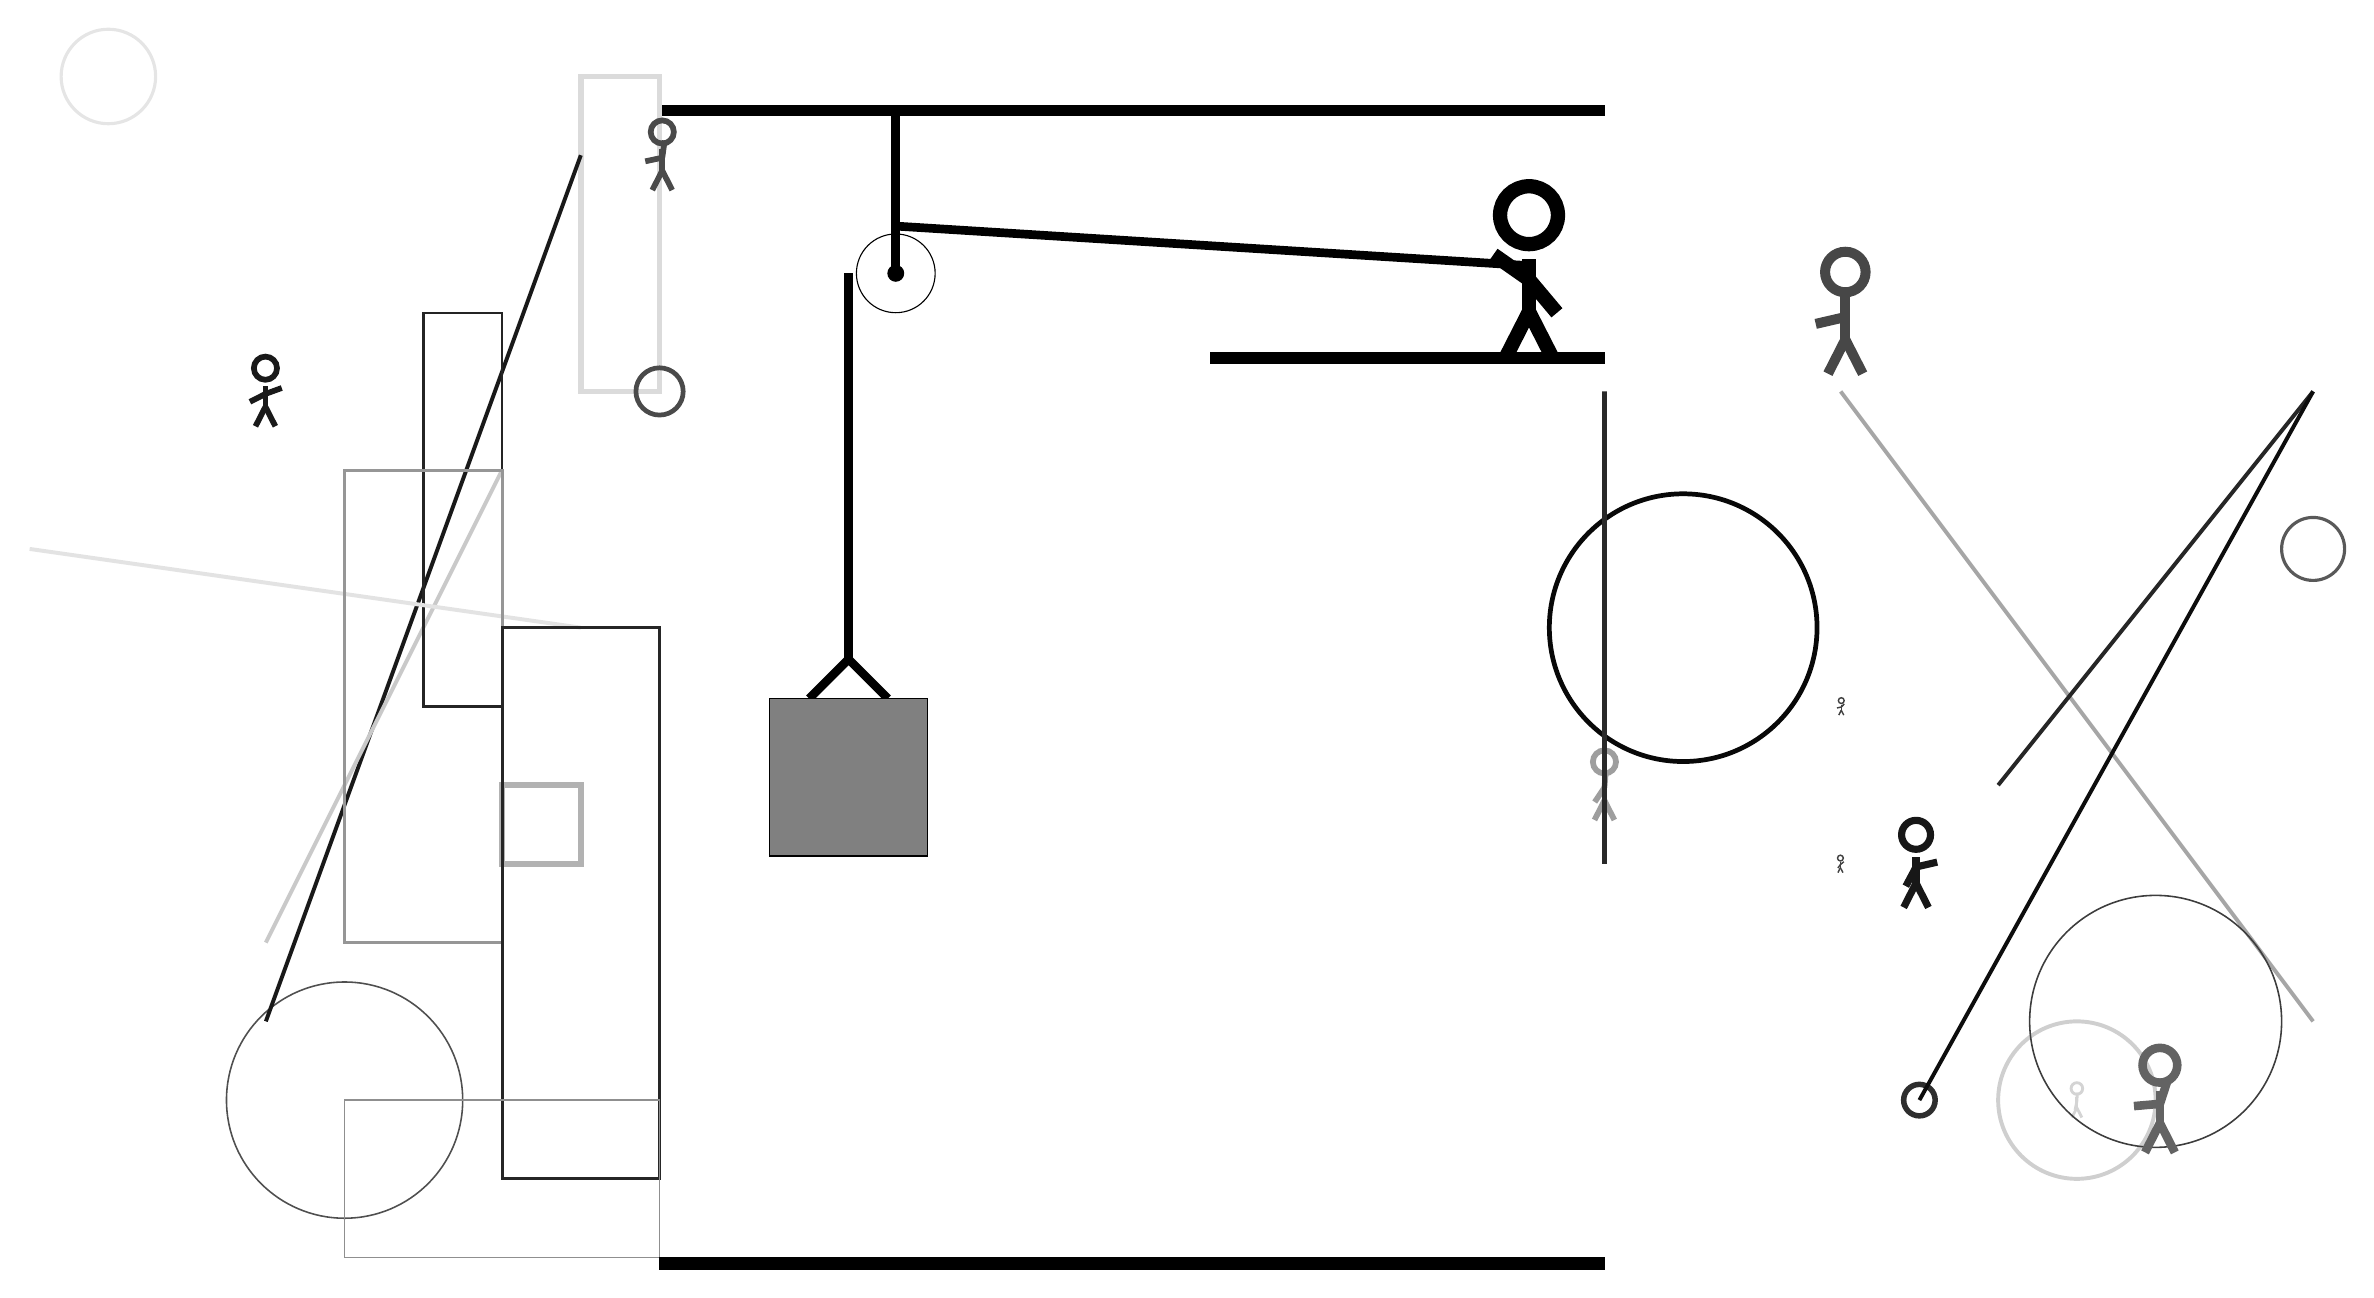
\begin{tikzpicture}
			%%%%% START %%%%%
			
			\draw[fill=black] (-2, 11.5) rectangle (10, 11.625);
			
			\draw (1, 9.5) circle (0.5);
			\draw[fill=black] (1, 9.5) circle (0.1);
			\draw[line width=1.1mm] (1, 11.5) -- (1, 9.5);
			
			\draw[line width=1.1mm](-0.1, 4.1) --  (0.4, 4.6) -- (0.9, 4.1);
			\draw[fill=black!50] (-0.6, 4.1) rectangle (1.4, 2.1);
			
			\node[line width=0.2mm, color=black!75] at (13, 4) {\Strichmaxerl[1][12][46]};
			
			\draw [line width=0.7mm, color=black!82](14, -1) circle (0.2);
			\node[line width=0.4mm, color=black!17] at (16, -1) {\Strichmaxerl[2][78][87]};
			\draw [line width=0.4mm, color=black!65](19, 6) circle (0.4);
			
			\draw[line width=0.7mm, color=black!14] (-2, 12) rectangle (-3, 8);
			\draw[line width=0.5mm, color=black!35](13, 8) -- (19, 0);
			
			\draw[line width=0.7mm, color=black!30] (-4, 2) rectangle (-3, 3);
			\draw [line width=0.5mm, color=black!19](16, -1) circle (1.0);
			\node[line width=0.4mm, color=black!91] at (14, 2) {\Strichmaxerl[5][62][13]};
			\node[line width=0.4mm, color=black!71] at (-2, 11) {\Strichmaxerl[4][12][82]};
			\node[line width=0.5mm, color=black!90] at (-7, 8) {\Strichmaxerl[4][27][20]};
			\draw [line width=0.2mm, color=black!69](-6, -1) circle (1.5);
			\draw [line width=0.2mm, color=black!76](17, 0) circle (1.6);
			
			\draw[line width=0.5mm, color=black!90](-7, 0) -- (-3, 11);
			\node[line width=0.4mm, color=black!74] at (13, 2) {\Strichmaxerl[1][54][39]};
			\node[line width=0.7mm, color=black!61] at (17, -1) {\Strichmaxerl[6][5][72]};
			\draw[line width=0.5mm, color=black!85](15, 3) -- (19, 8);
			
			\draw [line width=0.4mm, color=black!10](-9, 12) circle (0.6);
			\draw[line width=0.5mm, color=black!21](-7, 1) -- (-4, 7);
			\draw [line width=0.6mm, color=black!97](11, 5) circle (1.7);
			\draw [line width=0.6mm, color=black!71](-2, 8) circle (0.3);
			
			\draw[line width=0.3mm, color=black!86] (-4, 9) rectangle (-5, 4);
			
			\draw[line width=0.5mm, color=black!11](-3, 5) -- (-10, 6);
			\draw[line width=0.4mm, color=black!41] (-4, 7) rectangle (-6, 1);
			\node[line width=0.3mm, color=black!38] at (10, 3) {\Strichmaxerl[4][56][85]};
			
			\draw[line width=0.6mm, color=black!84] (10, 8) rectangle (10, 2);
			\draw[line width=0.5mm, color=black!95](14, -1) -- (19, 8);
			\draw[line width=0.4mm, color=black!85] (-4, -2) rectangle (-2, 5);
			\draw [line width=0.6mm, color=black!31](-7, 0) circle (0.0);
			\draw[line width=0.2mm, color=black!44] (-2, -1) rectangle (-6, -3);
			\node[line width=0.5mm, color=black!72] at (13, 9) {\Strichmaxerl[7][13][90]};
			
			
			\draw[line width=1.1mm](0.4, 9.5) -- (0.4, 4.6);
			\centerarc[line width=1.1mm](1, 9.5)(90:180:0.6)
			\draw[line width=1.1mm](1, 10.1) -- (9, 9.6);
			
			\node at (9, 9.5) {\Strichmaxerl[10][-35][-50]};
			\draw[fill=black] (5, 8.5) rectangle (10, 8.35);
			
			\draw[fill=black] (-2, -3) rectangle (10, -3.15);
			
			%%%%% END %%%%%
		\end{tikzpicture}
	\end{figure}	
\end{document}